%%%%% Set up %%%%%

% Set document style and font size
\documentclass[12pt]{article}\usepackage[]{graphicx}\usepackage[]{color}
%% maxwidth is the original width if it is less than linewidth
%% otherwise use linewidth (to make sure the graphics do not exceed the margin)
\makeatletter
\def\maxwidth{ %
  \ifdim\Gin@nat@width>\linewidth
    \linewidth
  \else
    \Gin@nat@width
  \fi
}
\makeatother

\definecolor{fgcolor}{rgb}{0.345, 0.345, 0.345}
\newcommand{\hlnum}[1]{\textcolor[rgb]{0.686,0.059,0.569}{#1}}%
\newcommand{\hlstr}[1]{\textcolor[rgb]{0.192,0.494,0.8}{#1}}%
\newcommand{\hlcom}[1]{\textcolor[rgb]{0.678,0.584,0.686}{\textit{#1}}}%
\newcommand{\hlopt}[1]{\textcolor[rgb]{0,0,0}{#1}}%
\newcommand{\hlstd}[1]{\textcolor[rgb]{0.345,0.345,0.345}{#1}}%
\newcommand{\hlkwa}[1]{\textcolor[rgb]{0.161,0.373,0.58}{\textbf{#1}}}%
\newcommand{\hlkwb}[1]{\textcolor[rgb]{0.69,0.353,0.396}{#1}}%
\newcommand{\hlkwc}[1]{\textcolor[rgb]{0.333,0.667,0.333}{#1}}%
\newcommand{\hlkwd}[1]{\textcolor[rgb]{0.737,0.353,0.396}{\textbf{#1}}}%
\let\hlipl\hlkwb

\usepackage{framed}
\makeatletter
\newenvironment{kframe}{%
 \def\at@end@of@kframe{}%
 \ifinner\ifhmode%
  \def\at@end@of@kframe{\end{minipage}}%
  \begin{minipage}{\columnwidth}%
 \fi\fi%
 \def\FrameCommand##1{\hskip\@totalleftmargin \hskip-\fboxsep
 \colorbox{shadecolor}{##1}\hskip-\fboxsep
     % There is no \\@totalrightmargin, so:
     \hskip-\linewidth \hskip-\@totalleftmargin \hskip\columnwidth}%
 \MakeFramed {\advance\hsize-\width
   \@totalleftmargin\z@ \linewidth\hsize
   \@setminipage}}%
 {\par\unskip\endMakeFramed%
 \at@end@of@kframe}
\makeatother

\definecolor{shadecolor}{rgb}{.97, .97, .97}
\definecolor{messagecolor}{rgb}{0, 0, 0}
\definecolor{warningcolor}{rgb}{1, 0, 1}
\definecolor{errorcolor}{rgb}{1, 0, 0}
\newenvironment{knitrout}{}{} % an empty environment to be redefined in TeX

\usepackage{alltt}

% File path to resources (style file etc)
\newcommand{\locRepo}{csas-style}

% Style file for DFO Technical Reports
\usepackage{\locRepo/tech-report}

% header-includes from R markdown entry
\usepackage{pdflscape}

%%%%% Variables %%%%%

% New definitions: Title, year, report number, authors
% Protect lower case words (i.e., species names) in \Addlcwords{}, in "TechReport.sty"
\newcommand{\trTitle}{Estimation of fork length using cranial measurements of sablefish (\emph{Anoplopoma fimbria}) in British Columbia.}
\newcommand{\trYear}{2021}
\newcommand{\trReportNum}{nnn}
% Optional
\newcommand{\trAuthFootA}{Email: \link{mailto:Kathryn.Temple@dfo-mpo.gc.ca}{\nolinkurl{Kathryn.Temple@dfo-mpo.gc.ca}} \textbar{} telephone: (250) 756-7366}
\newcommand{\trAuthsLong}{Kathryn x. Temple and Kendra R. Holt and Lisa C. Lacko}
\newcommand{\trAuthsBack}{Kathryn x. Temple, K.R. Holt and Lacko, L.C.}

% New definition: Address
\newcommand{\trAddy}{Pacific Biological Station\\
Fisheries and Oceans Canada, 3190 Hammond Bay Road\\
Nanaimo, British Columbia, V9T 6N7, Canada\\}

% Abstract
\newcommand{\trAbstract}{Routine biological sampling of whole round sablefish from commercial fishing operations in British Columbia have occurred since the early 1990's. Historically, specimens have been obtained through a voluntary catch sampling program and tagged sablefish recovery program. In order to improve the quantity and size range of samples received, we investigated the potential for obtaining biological information using heads, rather than the entire fish. In 2016, 438 sablefish (240-1080 mm) were sampled at sea and six different fish head measurements were assessed to see if they could predict fork length. Genetic samples (137) were collected to develop methods for DNA-based sex identification. A pilot study was conducted in 2017 with head-only samples and sex determination provided by a commercial vessel, followed by scientific sampling on shore. Regression analysis results show that the interorbital distance measurement was a good predictor of sablefish fork length, while samplers ranked it the most efficient and easily repeatable. Initial genetic samples (130/137) were successfully PCR amplified from genomic DNA and results indicate 92\% accuracy in sex detection. Subsequently, the 2018 sampling collection program was modified so that returns of whole round sablefish were replaced by head-only samples with knife cuts on the operculum to indicate sex.}

% Resume (i.e., French abstract)
\newcommand{\trResume}{Routine biological sampling of whole round sablefish from commercial fishing operations in British ColumbRoutine biological sampling of whole round sablefish from commercial fishing operations in British Columbia have occurred since the early 1990's. Historically, specimens have been obtained through a voluntary catch sampling program and tagged sablefish recovery program. In order to improve the quality of samples received, we investigated the potential for obtaining biological information using heads, rather than the entire fish. In 2016, 438 sablefish (240-1080 mm) were sampled at sea and six different fish head measurements were assessed to see if they could predict fork length. Genetic samples (137) were collected to develop methods for DNA-based sex identification. A pilot study was conducted in 2017 with head-only samples and sex determination provided by a commercial vessel, followed by scientific sampling on shore. Regression analysis results show that the interorbital distance measurement was a good predictor of sablefish fork length, while samplers ranked it the most efficient and easily repeatable. Initial genetic samples (130/137) were successfully PCR amplified from genomic DNA and results indicate 92\% accuracy in sex detection. Fisher sex determination was xx\%. Subsequently, the 2018 sampling collection program was modified so that returns of whole round sablefish were replaced by head-only samples with knife cuts on the operculum to indicate sex.}

\newcommand{\trISBN}{}

\DeclareGraphicsExtensions{.png,.pdf}
%%%%% Start %%%%%

% Start the document
\IfFileExists{upquote.sty}{\usepackage{upquote}}{}

% commands and environments needed by pandoc snippets
% extracted from the output of `pandoc -s`
%% Make R markdown code chunks work
\usepackage{array}
\usepackage{amssymb,amsmath}
\usepackage{color}
\usepackage{fancyvrb}

% From default template:
\newcommand{\VerbBar}{|}
\newcommand{\VERB}{\Verb[commandchars=\\\{\}]}
\DefineVerbatimEnvironment{Highlighting}{Verbatim}{commandchars=\\\{\},formatcom=\color[rgb]{0.00,0.00,0.00}}
\usepackage{framed}
\definecolor{shadecolor}{RGB}{248,248,248}
\newenvironment{Shaded}{\begin{snugshade}}{\end{snugshade}}
\newcommand{\AlertTok}[1]{\textcolor[rgb]{0.94,0.16,0.16}{#1}}
\newcommand{\AnnotationTok}[1]{\textcolor[rgb]{0.56,0.35,0.01}{\textbf{\textit{#1}}}}
\newcommand{\AttributeTok}[1]{\textcolor[rgb]{0.77,0.63,0.00}{#1}}
\newcommand{\BaseNTok}[1]{\textcolor[rgb]{0.00,0.00,0.81}{#1}}
\newcommand{\BuiltInTok}[1]{#1}
\newcommand{\CharTok}[1]{\textcolor[rgb]{0.31,0.60,0.02}{#1}}
\newcommand{\CommentTok}[1]{\textcolor[rgb]{0.56,0.35,0.01}{\textbf{#1}}}
\newcommand{\CommentVarTok}[1]{\textcolor[rgb]{0.56,0.35,0.01}{\textbf{\textit{#1}}}}
\newcommand{\ConstantTok}[1]{\textcolor[rgb]{0.00,0.00,0.00}{#1}}
\newcommand{\ControlFlowTok}[1]{\textcolor[rgb]{0.13,0.29,0.53}{\textit{#1}}}
\newcommand{\DataTypeTok}[1]{\textcolor[rgb]{0.13,0.29,0.53}{#1}}
\newcommand{\DecValTok}[1]{\textcolor[rgb]{0.00,0.00,0.81}{#1}}
\newcommand{\DocumentationTok}[1]{\textcolor[rgb]{0.56,0.35,0.01}{\textbf{\textit{#1}}}}
\newcommand{\ErrorTok}[1]{\textcolor[rgb]{0.64,0.00,0.00}{\textit{#1}}}
\newcommand{\ExtensionTok}[1]{#1}
\newcommand{\FloatTok}[1]{\textcolor[rgb]{0.00,0.00,0.81}{#1}}
\newcommand{\FunctionTok}[1]{\textcolor[rgb]{0.00,0.00,0.00}{#1}}
\newcommand{\ImportTok}[1]{#1}
\newcommand{\InformationTok}[1]{\textcolor[rgb]{0.56,0.35,0.01}{\textbf{\textit{#1}}}}
\newcommand{\KeywordTok}[1]{\textcolor[rgb]{0.13,0.29,0.53}{\textit{#1}}}
\newcommand{\NormalTok}[1]{#1}
\newcommand{\OperatorTok}[1]{\textcolor[rgb]{0.81,0.36,0.00}{\textit{#1}}}
\newcommand{\OtherTok}[1]{\textcolor[rgb]{0.56,0.35,0.01}{#1}}
\newcommand{\PreprocessorTok}[1]{\textcolor[rgb]{0.56,0.35,0.01}{\textbf{#1}}}
\newcommand{\RegionMarkerTok}[1]{#1}
\newcommand{\SpecialCharTok}[1]{\textcolor[rgb]{0.00,0.00,0.00}{#1}}
\newcommand{\SpecialStringTok}[1]{\textcolor[rgb]{0.31,0.60,0.02}{#1}}
\newcommand{\StringTok}[1]{\textcolor[rgb]{0.31,0.60,0.02}{#1}}
\newcommand{\VariableTok}[1]{\textcolor[rgb]{0.00,0.00,0.00}{#1}}
\newcommand{\VerbatimStringTok}[1]{\textcolor[rgb]{0.31,0.60,0.02}{#1}}
\newcommand{\WarningTok}[1]{\textcolor[rgb]{0.56,0.35,0.01}{\textbf{\textit{#1}}}}
\begin{document}

%%%% Front matter %%%%%

% Add the first few pages
\frontmatter

%%%%% Drafts %%%%%

%\linenumbers  % Line numbers
%\onehalfspacing  % Extra space between lines
\renewcommand{\headrulewidth}{0.5pt}  % Header line
\renewcommand{\footrulewidth}{0.5pt}  % footer line
%\pagestyle{fancy}\fancyhead[c]{Draft: Do not cite or circulate}  % Header text

\newcommand{\lt}{\ensuremath <}
\newcommand{\gt}{\ensuremath >}

%Defines cslreferences environment
%Required by pandoc 2.8
%Copied from https://github.com/rstudio/rmarkdown/issues/1649
\newlength{\cslhangindent}
\setlength{\cslhangindent}{1.5em}
\newenvironment{cslreferences}%
  {}%
  {\par}

%%%%% Main document %%%%%
\hypertarget{introduction}{%
\section{Introduction}\label{introduction}}

Biological samples of British Columbia (BC) sablefish (\emph{Anoplopoma fimbria}) have been collected from a voluntary catch sampling program since 1995 (\protect\hyperlink{ref-Haist2001}{Haist and Wyeth 2001}) and processed by the Department of Fisheries and Oceans (DFO) port samplers and contracted service providers. In addition, whole tagged fish recovered in commercial fisheries (trap, trawl, hook and line) have been received at the point of landing via the dockside monitoring program (DMP) and sampled by Archipelago Marine Research (AMR) since the early 1990's. These data provide a fishery dependent source of age and size composition data for the two-sex structured operating model of the coastal Management Strategy Evaluation (MSE) (\protect\hyperlink{ref-Cox2019}{Cox et al. 2019}).

In recent years, a sablefish head only catch sampling and tagging program was developed in order to improve the number of returns, maintain the quality of the biological data and increase the range of fish sizes. Instead of returning the whole fish, commercial crew j-cut the fish as per commercial practice, view the gonads to determine sex, mark the sex with knife cuts on the operculum and store the head (and/or floy tag) for later sampling by the department and AMR.

Previous research has accurately estimated fish lengths from i) head measurements (\protect\hyperlink{ref-Serafy1996}{Serafy et al. 1996}; \protect\hyperlink{ref-Park2019}{Park et al. 2019}), ii) head and mandible lengths (\protect\hyperlink{ref-Isermann2005}{Isermann and Vandergoot 2005}) and iii) relative eye size (\protect\hyperlink{ref-Richardson2015}{Richardson et al. 2015}). In our research, six unique sablefish head dimensions including fork length (FL), eye diameter (ED), interorbital distance (ID), snout length (SL), post orbital to preoperculum distance (PP) and post orbital head length (PO) were regressed against fork length (FL). In addition, a task performance ranking system was developed to reveal the most accurate and efficient cranial measurement.

In 2016, standard biological data including operculum clips (DNA) were obtained on several research surveys from 216 female and 222 male sablefish, followed by cranial measurements at the Pacific Biological Station (PBS). Methods for DNA-based sex identification were developed by the PBS Molecular Genetics lab. In 2017, a pilot study was conducted on a commercial vessel. Head-only samples with sex markings were collected at sea, followed by scientific sampling on shore. DNA analysis measured the commercial fisher sex accuracy.

In this technical report we describe the results of 1) the relationship between head measurements and fork length; 2) the feasibility of the head measurements; 3) the methods of DNA sex detection; and 4) the fisher-determined sex accuracy via genetic methods. Successful application of this research has resulted in program revisions in the catch sampling programs and shore-side sampling of sablefish in 2018.

\hypertarget{methods}{%
\section{Methods}\label{methods}}

\hypertarget{experimental-study-2016}{%
\subsection{Experimental Study 2016}\label{experimental-study-2016}}

\hypertarget{sample-collection}{%
\subsubsection{Sample collection}\label{sample-collection}}

Sablefish were selected for sampling during the 2016 biennial DFO Groundfish Synoptic Bottom Trawl surveys, following a trip-wide length stratified selection protocol. A tally of 212 fish were sampled on the West Coast Vancouver Island survey (\protect\hyperlink{ref-Williams2018}{Williams et al. 2018}) and 219 fish were sampled on the West Coast Haida Gwaii survey (\protect\hyperlink{ref-Nottingham2018}{Nottingham et al. 2018}). In addition, seven small sablefish were collected during the 2016 salmon survey (Figure~\ref{fig:figure1}).

For each selected fish, fork length, round weight, fish sex and maturity (determined by internal examination of the gonads) were recorded at sea. The heads were removed, tagged and frozen. On shore, cranial dimensions were measured using Mitutoyo Absolute® 500-762-20 coolant proof digimatic calipers. Ageing structures (sagittal otoliths) were also collected from each head. Operculum clips (DNA) were collected from the first 137 fish measured (79 male and 58 female), and stored in vials containing 95\% ethanol.

\hypertarget{estimation-of-fork-length-using-cranial-measurements}{%
\subsubsection{Estimation of Fork Length using Cranial Measurements}\label{estimation-of-fork-length-using-cranial-measurements}}

A number of cranial dimensions were considered as possible candidates for estimating fork length: upper jaw length (UJ), eye diameter (ED), interorbital distance (ID), snout length (SL), post orbital to preoperculum distance (PP), and post orbital (PO) head length (Table~\ref{tab:table1}; Appendix~\ref{app:second-appendix}). The head length to fork length relationships were calculated by linear regression.

Each cranial dimension was ranked by samplers on a five point rating scale in terms of ease of use and repeatability with electronic calipers. The ease of use metric focused on three key attributes of the measurement learnability (task understanding), efficiency (task-completion time) and degree of difficulty (task performance ease). The repeatability metric focused on ranking each measurement under repeated caliper placement, taking into consideration the soft and hard head tissues.

\hypertarget{genetic-test-development-for-gender-determination}{%
\subsubsection{Genetic test development for gender determination}\label{genetic-test-development-for-gender-determination}}

DNA multiplex polymerase chain reactions (PCRs) were conducted using fluorescently labelled forward primers. X-insert and Y-insert specific primers developed by \protect\hyperlink{ref-Rondeau2013}{Rondeau et al.} (\protect\hyperlink{ref-Rondeau2013}{2013}) were used, but the X-insert forward and Y-nested reverse were redesigned to produce slightly smaller PCR products (Table~\ref{tab:table2}). Sex specific alleles were size fractionated in an ABI 3730 capillary DNA analyzer and were scored with ABI GeneMapper using an internal lane sizing standard.

\hypertarget{pilot-study-2017}{%
\subsection{Pilot study 2017}\label{pilot-study-2017}}

In 2017, a pilot study was conducted with the commercial sector returning sablefish head only samples. A total of 360 heads were collected from J-cut sablefish on a limited-entry fishery trip to the S\(\text{\underline{G}}\)aan \(\text{\underline{K}}\)inghlas - Bowie (SK-B) seamount. Each operculum was marked by commercial fishers with either one knife cut (male) or two knife cuts (female) (Appendix~\ref{app:second-appendix}). Scientific sampling occurred on shore, with the first 99 heads of the pilot study measured by three technicians for ID, SL, UJ and PP. Fin clips were forwarded to the molecular genetics lab for sex determination.

\clearpage

\hypertarget{results-and-discussion}{%
\section{Results and Discussion}\label{results-and-discussion}}

\hypertarget{experimental-study-2016-1}{%
\subsection{Experimental Study 2016}\label{experimental-study-2016-1}}

A total of 438 specimens comprising 222 males and 216 females were used for the study. The smallest fork length of the collected specimens was 240 mm, the highest was 1080 mm, and an average of 573.2990868 (Table~\ref{tab:table3}).

The mean values of the predictor and response variables collected for five of the six head measurements (UJ, ED, IO, SL, PP, PH)(Table~\ref{tab:table2}). The PH head was abandoned after 130 sablefish due to the time consuming and technical difficulties performing this measurement.

We found evidence of relationships between upper jaw length and fork length (p = \ensuremath{9.358\times 10^{-278}}) ; eye diameter and fork length (p = \ensuremath{5.34\times 10^{-203}}); interorbital distance and fork length (p = \ensuremath{5.539\times 10^{-272}} ); upper snout length and fork length (p = \ensuremath{4.593\times 10^{-292}}); postorbital to preoperculum length and fork length (p = \ensuremath{2.024\times 10^{-247}}); and postorbital head length and fork length (p = 0).

, fork length, round weight, otoliths and DNA. Post orbital head length (Posterior inner edge of orbit to dorsal insertion of opercle) was also measured, but this was abandoned after 130 measurements, to save time, and because it was not possible to measure this on a number of the heads for a variety of reasons (opercula had been cut off from some heads, it was awkward to take longer measurements using the electronic calipers, and the end points of the measurement were difficult to define.

\hypertarget{estimation-of-fork-length-using-cranial-measurements-1}{%
\subsection{Estimation of Fork Length using Cranial Measurements}\label{estimation-of-fork-length-using-cranial-measurements-1}}

Given the ease of measurement, we suggest that Interorbital distance be used to predict sablefish fork lengths and weights (Table~\ref{tab:table3}).

The estimated slope is 7.695 (SE 0.088) units of fork length per unit of upper jaw length; the estimated slope is 21.994 (SE 0.389) units of fork length per unit of eye diameter; the estimated slope is 11.622 (SE 0.138) units of fork length per unit of interorbital distance; the estimated slope is 11.182 (SE 0.118 units of fork length per unit of snout length; the estimated slope is 14.373 (SE 0.191) units of fork length per unit of postorbital to preoperculum length; and the estimated slope is 6.83 (SE 0.185) units of fork length per unit of postorbital head length.

\hypertarget{pilot-collection-of-sablefish-heads-as-a-biological-sample}{%
\subsection{Pilot Collection of Sablefish Heads as a Biological Sample}\label{pilot-collection-of-sablefish-heads-as-a-biological-sample}}

Heads were received by DFO in good condition (intact and not deformed), segregated by set, for measuring and otolith extraction. Operculum cuts worked well to indicate sex

\hypertarget{repeatability-of-measurements-between-technicians}{%
\subsection{Repeatability of measurements between technicians}\label{repeatability-of-measurements-between-technicians}}

\hypertarget{discussion}{%
\section{Discussion}\label{discussion}}

Routine biological sampling procedures have been modified so that commercial fisheries are now only returning heads, rather than entire fish.

\clearpage

\hypertarget{tables}{%
\section{Tables}\label{tables}}



\begin{table}[!h]

\caption{\label{tab:table1}List of head dimensions, measurement descriptions and specification of caliper jaw placement. ~\\
\hspace*{0.333em}\\}
\fontsize{10}{12}\selectfont
\begin{tabular}[t]{>{\raggedright\arraybackslash}p{1.9cm}>{\raggedright\arraybackslash}p{6.0cm}>{\raggedright\arraybackslash}p{7.5cm}}
\toprule
\textbf{Head dimension} & \textbf{Head description} & \textbf{Caliper jaw position}\\
\midrule
UJ & Tip of snout to the posterior edge of the maxilla. & Outside caliper jaw measurement from forward point and centre of snout to back of maxilla.\\
\midrule
ED & Anterior-posterior diameter of eye socket. & Inside caliper jaw measurement firmly stretched against eye socket at vertical midpoint of eye.\\
\midrule
ID & Narrowest distance between eye sockets, measured on dorsal surface. & Outside caliper jaw measurement of the horizontal midpoint of eyes on dorsal surface.\\
\midrule
SL & Tip of snout to anterior inner edge of eye socket. & Outside caliper jaw measurement from forward point and centre of snout to horizontal midpoint of anterior edge of eye socket.\\
\midrule
PP & Posterior inner edge of orbit to visual insertion point of preopercle. & Outside caliper jaw measurement from back of eye socket to preopercle bone insertion point. Preopercle must be lifted to expose preopercle bone underneath.\\
\midrule
\addlinespace
PO & Posterior inner edge of orbit to dorsal insertion of opercle. & Outside caliper jaw measurement from back of eye socket to bone underneath gill cover notch at dorsal insertion of the opercle.  The operculum must be held taut.\\
\bottomrule
\end{tabular}
\end{table}
~\\
\hspace*{0.333em}\\


\begin{table}[!h]

\caption{\label{tab:table2}Primers used in the development of a genetic test for determining sablefish sex. ~\\
\hspace*{0.333em}\\}
\fontsize{10}{12}\selectfont
\begin{tabular}[t]{llr}
\toprule
\textbf{Locus} & \textbf{Sequence} & \textbf{Fragment.Size}\\
\midrule
X-insert-DFO\_F1 & 6FAM-CACCGCTCATGTACACTTTG & 321\\
X-insert-2R & TGCTGCACTGTACCATCAAA & \\
Y-nested-1F & NED-GTCAGAAGGCAGTGGTGTAGT & 234\\
Y-nested-MGL\_2R & CGCTTGCAGATACTACTGAATG & \\
\bottomrule
\end{tabular}
\end{table}
~\\
\hspace*{0.333em}\\


\begin{table}[!h]

\caption{\label{tab:table3}Summary of sablefish biological data collected. Tally of fork lengths (FL), round weight (RW), upper jaw length (UJ), eye diameter (ED), interorbital distance (ID), snout length (SL), post orbital to preoperculum distance (PP), post orbital head length (PO), females (F), males (M), sagittal otoliths and operculum clips (DNA) are listed by survey. ~\\
\hspace*{0.333em}\\}
\fontsize{10}{12}\selectfont
\begin{tabular}[t]{llllllllllllll}
\toprule
\textbf{Survey} & \textbf{FL} & \textbf{RW} & \textbf{UJ} & \textbf{ED} & \textbf{ID} & \textbf{SL} & \textbf{PP} & \textbf{PO} & \textbf{F} & \textbf{M} & \textbf{Otoliths} & \textbf{DNA} & \textbf{Total}\\
\midrule
2016 WCHG & 219 & 219 & 219 & 219 & 218 & 219 & 207 & 52 & 111 & 108 & 219 & 59 & 219\\
2016 WCVI & 212 & 212 & 211 & 212 & 212 & 211 & 212 & 78 & 105 & 107 & 212 & 78 & 212\\
Salmon & 7 & 0 & 7 & 7 & 7 & 7 & 7 & 0 & 0 & 7 & 0 & 0 & 7\\
\midrule
Total & 438 & 431 & 437 & 438 & 437 & 437 & 426 & 0 & 216 & 222 & 431 & 137 & 438\\
\bottomrule
\end{tabular}
\end{table}

\begin{table}[!h]

\caption{\label{tab:table4}Table of sample size, mean and standard deviation for predictor and response variables for each head dimension. ~\\}
\fontsize{10}{12}\selectfont
\begin{tabular}[t]{>{\raggedright\arraybackslash}p{5.9cm}>{\raggedright\arraybackslash}p{0.6cm}>{\raggedright\arraybackslash}p{0.6cm}>{\raggedright\arraybackslash}p{1.6cm}>{\raggedright\arraybackslash}p{2.1cm}>{\raggedright\arraybackslash}p{0.8cm}>{\raggedright\arraybackslash}p{0.6cm}}
\toprule
\textbf{Predictor variable} & \textbf{n} & \textbf{mean} & \textbf{sd} & \textbf{Response variable} & \textbf{mean} & \textbf{sd}\\
\midrule
Upper jaw length (UJ) & 437 & 57.95 & 15.22 & Fork length & 573.27 & 120.44\\
Eye diameter (ED) & 438 & 25.9 & 5.13 & Fork length & 573.3 & 120.3\\
InterOrbital distance (ID) & 437 & 40.37 & 10.06 & Fork length & 573.36 & 120.43\\
Snout length (SL) & 437 & 44.81 & 10.52 & Fork length & 573.27 & 120.44\\
Post orbital to preoperculum length (PP) & 426 & 31.5 & 8.02 & Fork length & 571.34 & 119.54\\
Post orbital head length (PO) & 130 & 60.85 & 18.87 & Fork length & 566.46 & 134.8\\
\bottomrule
\end{tabular}
\end{table}

\begin{table}

\caption{\label{tab:table5}Ease of use and repeat ability considerations for each measurement.number, ease of use and repeatability five point ranking where 5-Great; 4- Good; 3-Moderate; 2-Questionable; 1-Terrible.}
\fontsize{10}{12}\selectfont
\begin{tabular}[t]{>{\raggedright\arraybackslash}p{1.0cm}>{\raggedleft\arraybackslash}p{0.6cm}>{\raggedleft\arraybackslash}p{1.7cm}>{\raggedright\arraybackslash}p{1.2cm}>{\raggedright\arraybackslash}p{1.7cm}>{\raggedright\arraybackslash}p{1.7cm}>{\raggedright\arraybackslash}p{4.2cm}}
\toprule
\multicolumn{1}{c}{\textbf{ }} & \multicolumn{2}{c}{\textbf{5 Point}} & \multicolumn{1}{c}{\textbf{ }} & \multicolumn{2}{c}{\textbf{Measurement}} & \multicolumn{1}{c}{\textbf{ }} \\
\cmidrule(l{3pt}r{3pt}){2-3} \cmidrule(l{3pt}r{3pt}){5-6}
Head Dimension & Ease of use & Repeatable & Caliper limitation & Bilateral & Bone & Considerations\\
\midrule
UJ & 3 & 4 & x & x & x & End of the maxilla difficult to define. Caliper jaw position must be in center of snout.\\
\midrule
ED & 3 & 2 &  & x &  & Caliper outside jaw position on soft tissue in eye socket may result in measurement differences.\\
\midrule
ID & 5 & 5 &  &  & x & Tissue is compressed to obtain bone measurement. Easy to determine caliper jaw position.\\
\midrule
SL & 4 & 5 &  & x & x & Caliper jaw position must be in center of snout.\\
\midrule
PP & 4 & 5 &  & x & x & Caliper position on pre-operculum may result in measurement differences.\\
\midrule
PO & 3 & 2 & x & x &  & Operculum damage from handling was observed on several fish.\\
\bottomrule
\end{tabular}
\end{table}

\begin{table}

\caption{\label{tab:table6}Ease of use and repeat ability considerations for each measurement.number, ease of use and repeatability five point ranking where 5-Great; 4- Good; 3-Moderate; 2-Questionable; 1-Terrible.}
\fontsize{10}{12}\selectfont
\begin{tabular}[t]{lll}
\toprule
\textbf{Head dimension} & \textbf{slope} & \textbf{SE}\\
\midrule
Upper jaw length & 7.6946 & 0.088\\
Eye diameter & 21.994 & 0.389\\
InterOrbital distance & 11.622 & 0.138\\
Snout length & 11.182 & 0.118\\
Post orbital to preoperculum length & 14.373 & 0.191\\
Post orbital head length & 6.8299 & 0.185\\
\bottomrule
\end{tabular}
\end{table}
\clearpage

\hypertarget{figures}{%
\section{Figures}\label{figures}}


\begin{figure}[htb]

{\centering \pdftooltip{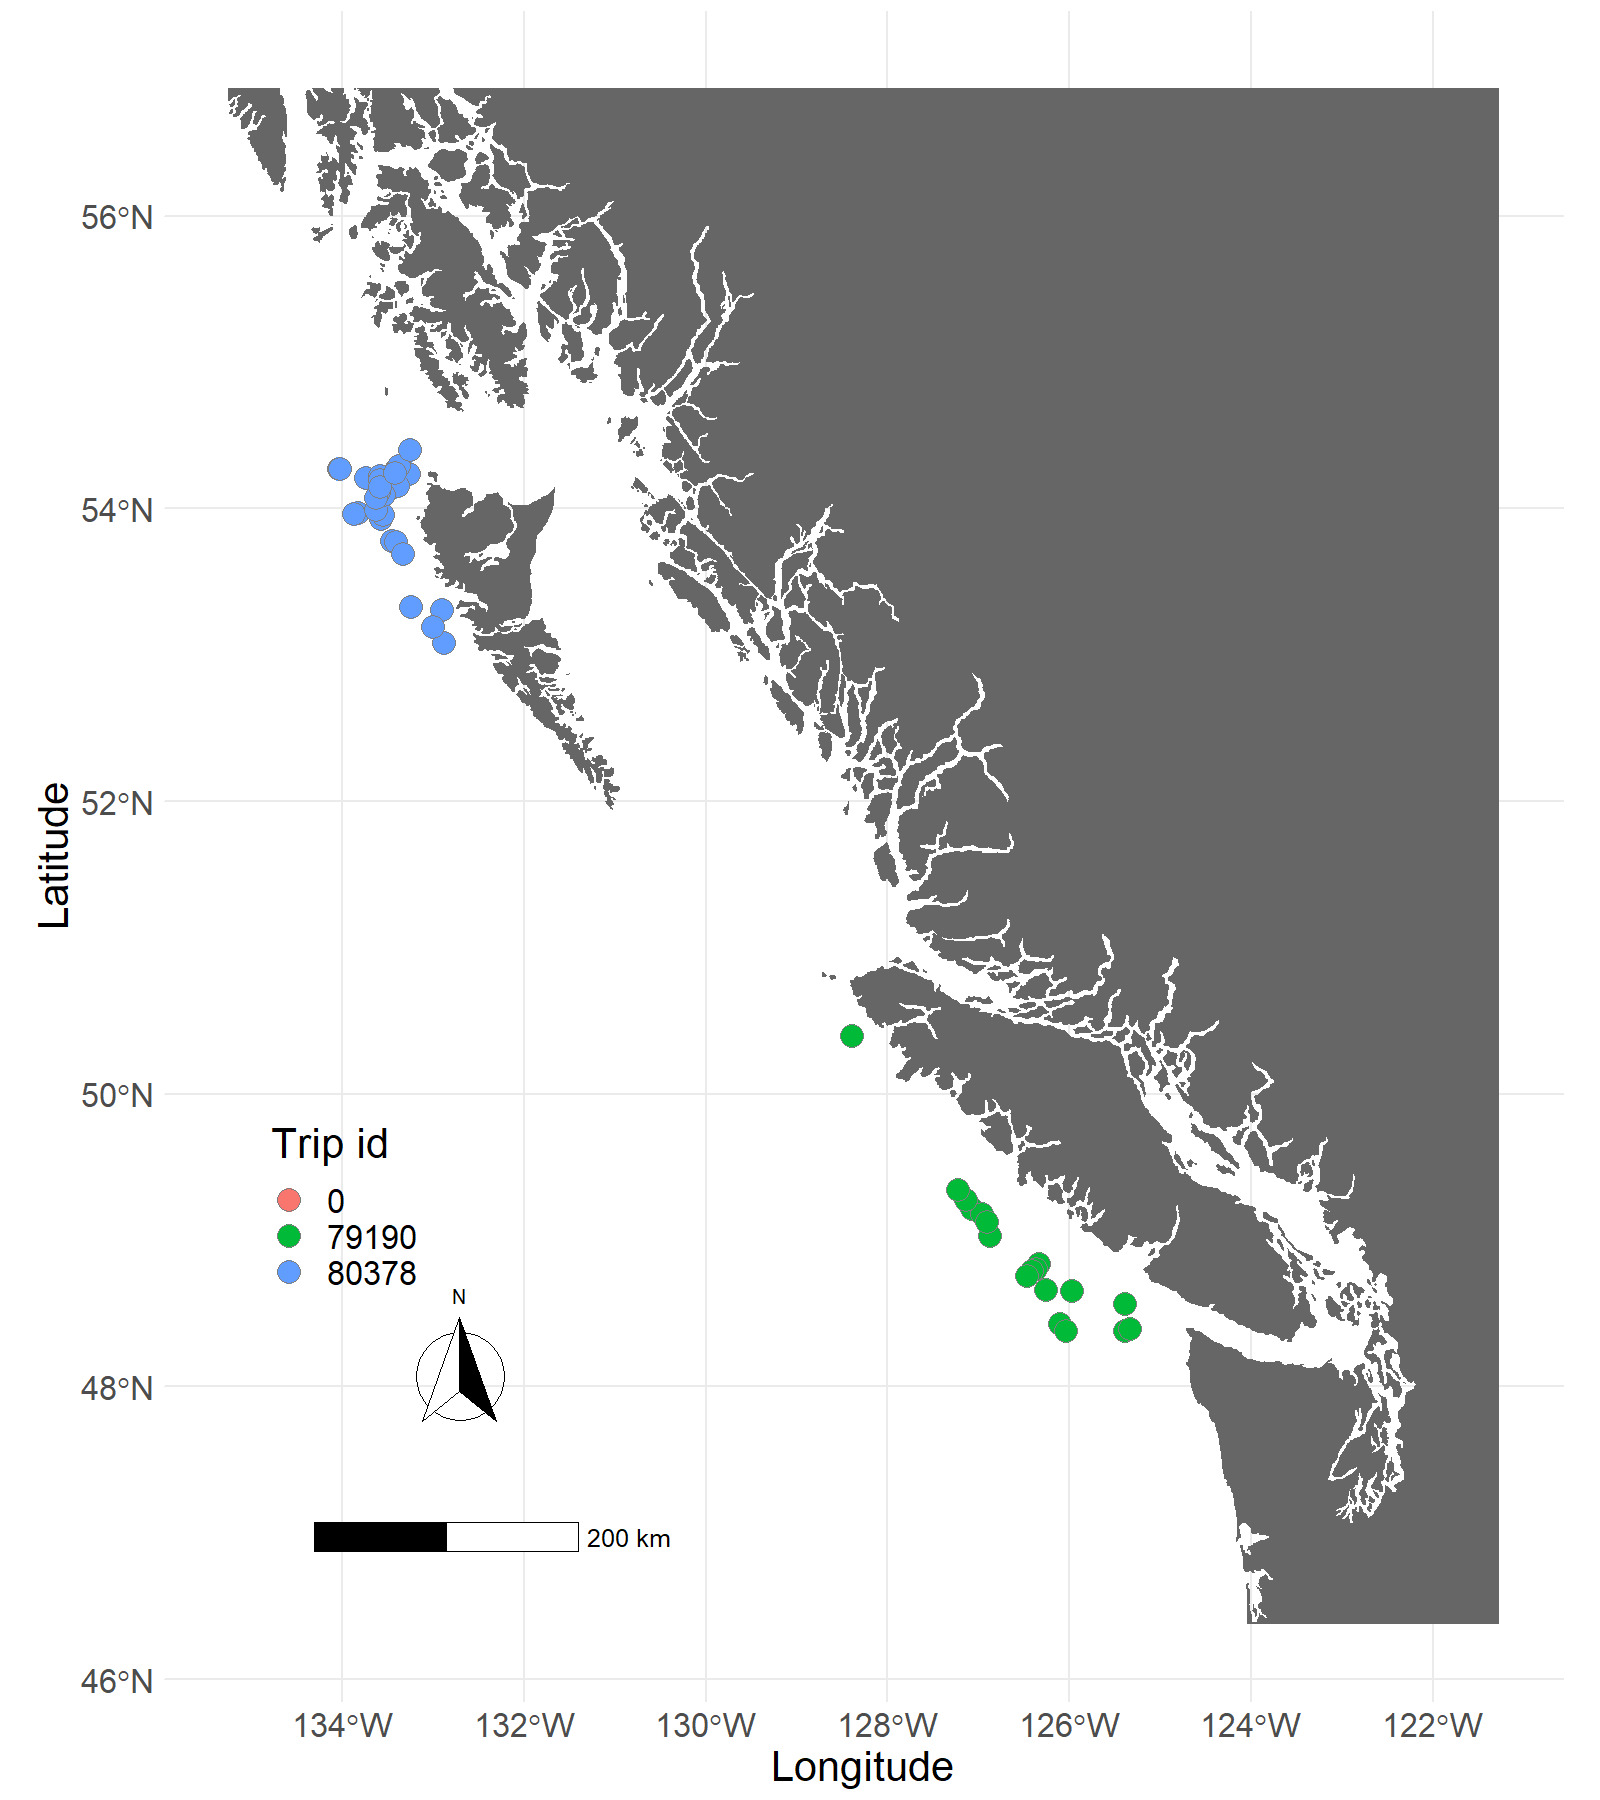
\includegraphics[width=6in]{C:/github/sablehead/figures/Figure1}}{Figure \ref{fig:figure1}} 

}

\caption{Sample locations in 2016 from the WCVI survey (GFBIO trip id 79190), WCHG survey (GFBIO trip id 80378) and salmon survey (?).}\label{fig:figure1}
\end{figure}

\begin{figure}[htb]

{\centering \pdftooltip{\includegraphics[width=400px,height=290px]{C:/github/sablehead/figures/figure2}}{Figure \ref{fig:figure2}} 

}

\caption{Scatterplot upper jaw vs fork length, measurements in millimeters.}\label{fig:figure2}
\end{figure}

\begin{figure}[htb]

{\centering \pdftooltip{\includegraphics[width=400px,height=290px]{C:/github/sablehead/figures/figure3}}{Figure \ref{fig:figure3}} 

}

\caption{Scatterplot eye diameter vs fork length, measurements in millimeters.}\label{fig:figure3}
\end{figure}

\begin{figure}[htb]

{\centering \pdftooltip{\includegraphics[width=400px,height=290px]{C:/github/sablehead/figures/figure4}}{Figure \ref{fig:figure4}} 

}

\caption{Scatterplot interorbital vs fork length.}\label{fig:figure4}
\end{figure}

\begin{figure}[htb]

{\centering \pdftooltip{\includegraphics[width=400px,height=290px]{C:/github/sablehead/figures/figure5}}{Figure \ref{fig:figure5}} 

}

\caption{Scatterplot snout length vs fork length.}\label{fig:figure5}
\end{figure}

\begin{figure}[htb]

{\centering \pdftooltip{\includegraphics[width=400px,height=290px]{C:/github/sablehead/figures/figure6}}{Figure \ref{fig:figure6}} 

}

\caption{Scatterplot post orbital to preoperculum length vs fork length.}\label{fig:figure6}
\end{figure}

\begin{figure}[htb]

{\centering \pdftooltip{\includegraphics[width=400px,height=290px]{C:/github/sablehead/figures/figure7}}{Figure \ref{fig:figure7}} 

}

\caption{Scatterplot of post orbital length vs fork length.}\label{fig:figure7}
\end{figure}
\clearpage

\begin{appendices}
\counterwithin{figure}{section}
\counterwithin{table}{section}
\counterwithin{equation}{section}

\clearpage

\section{IMAGES OF THE SIX CRANIAL DIMENSION MEASUREMENTS.}
\label{app:first-appendix}

A. Upper jaw measurement (UJ); B. Eye diameter measurement (ED); C. Interorbital distance (ID); D. Snout length (SL); E. Post orbital to preoperculum length measurement (PP); F. Post orbital head length (PO).
\begin{center}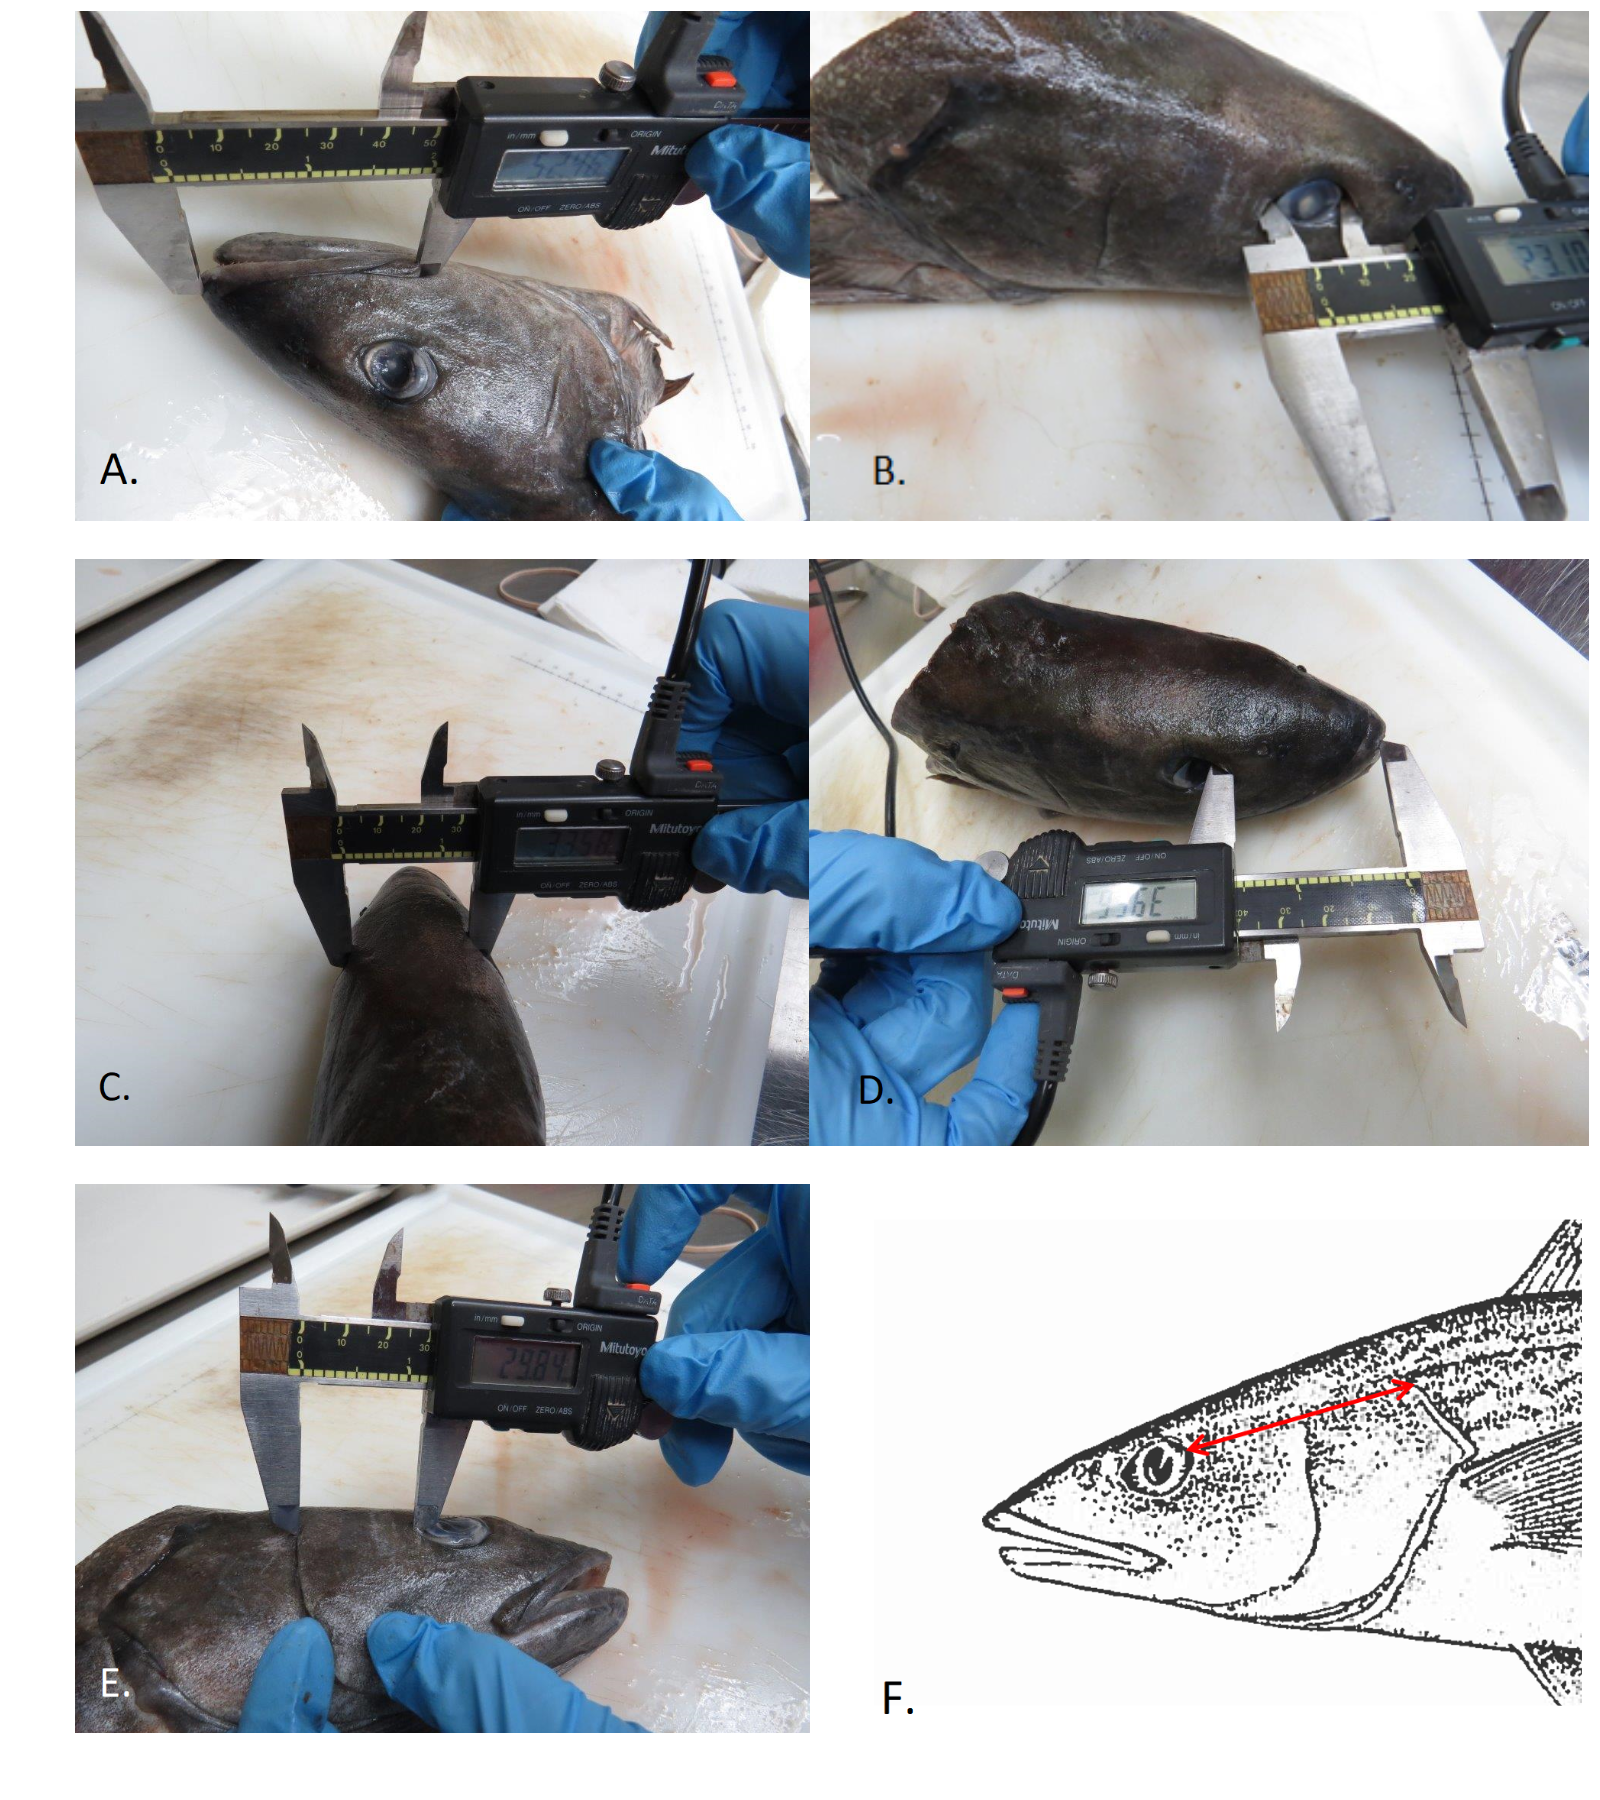
\includegraphics[width=6in]{C:/github/sablehead/figures/AppendixA} \end{center}

\clearpage

\section{SEX DETERMINATION BY OPERCULUM MARKING}
\label{app:second-appendix}

Operculum knife cuts for sablefish males (A) and females (B).
\begin{center}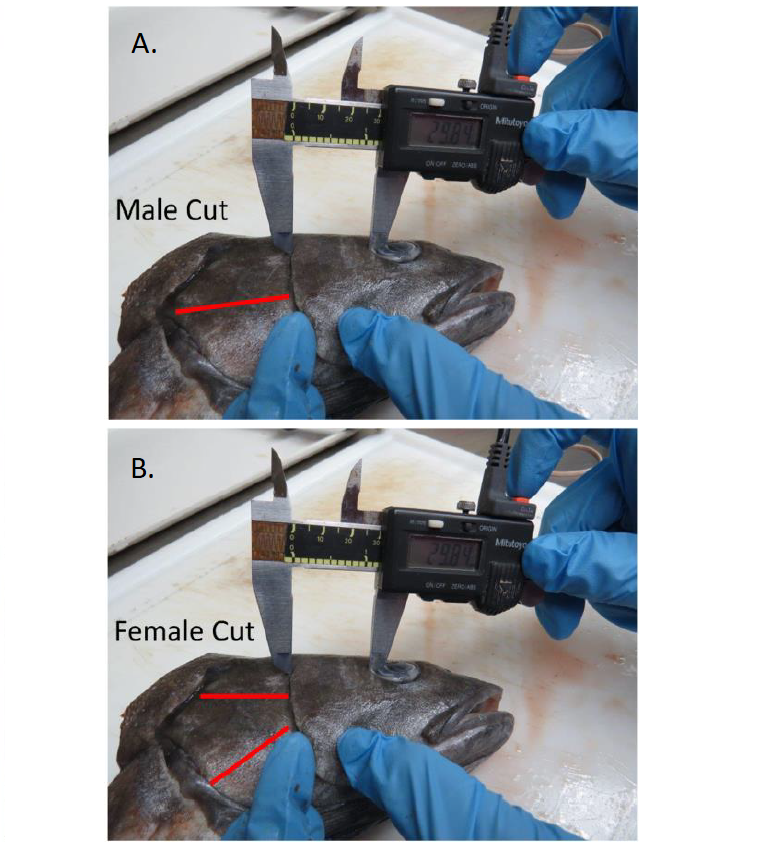
\includegraphics[width=6in]{C:/github/sablehead/figures/AppendixB} \end{center}
\clearpage

\end{appendices}

\clearpage

\hypertarget{references}{%
\section{References}\label{references}}

\noindent \vspace{-2em} \setlength{\parindent}{-0.2in} \setlength{\leftskip}{0.2in} \setlength{\parskip}{8pt}

\hypertarget{refs}{}
\begin{CSLReferences}{1}{0}
\leavevmode{\hypertarget{ref-Cox2019}{}}%
Cox, S.P., Holt, K., and Johnson, S. 2019. Evaluating the robustness of management procedures for the {Sablefish} (*anoplopoma fimbria*) fishery in {British Columbia, Canada} for 2017-18. DFO Can. Sci. Advis. Sec. Res. Doc. 2019/032. vi + 79 p.

\leavevmode{\hypertarget{ref-Haist2001}{}}%
Haist, R.H., V., and Wyeth, M. 2001. Sablefish {Stock Assessment} for 2001 and {Advice to Managers} for 2002. DFO Can. Sci. Advis. Sec. Res. Doc. 2001/135.

\leavevmode{\hypertarget{ref-Isermann2005}{}}%
Isermann, D.A., and Vandergoot, C.S. 2005. Predicting walleye total length from head and mandible measurements. North American Journal of Fisheries Management 25(1): 316--321. Taylor \& Francis.

\leavevmode{\hypertarget{ref-Nottingham2018}{}}%
Nottingham, M.K., Williams, D.C., Wyeth, M.R., and Olsen, N. 2018. Summary of the west coast haida gwaii synoptic bottom trawl survey, august 25 - september 26, 2016. Can. Manuscr. Rep. Fish. Aquat. Sci. 3151: viii: 51 p.

\leavevmode{\hypertarget{ref-Park2019}{}}%
Park, I.-S., Kim, Y.J., Choi, H.J., Oh, S.-Y., Noh, C.H., and Lee, S.-H. 2019. Total length estimation from head dimensions of artificially propagated brown croaker miichthys miiuy.

\leavevmode{\hypertarget{ref-Richardson2015}{}}%
Richardson, J., Shears, N., and Taylor, R. 2015. Using relative eye size to estimate the length of fish from a single camera image. Marine Ecology Progress Series 538.

\leavevmode{\hypertarget{ref-Rondeau2013}{}}%
Rondeau, E.B., Messmer, A.M., Sanderson, D.S., Jantzen, S.G., Schalburg, K.R. von, Minkley, D.R., Leong, J.S., Macdonald, G.M., Davidsen, A.E., Parker, W.A., Mazzola, R.S.A., Campbell, B., and Koop, B.F. 2013. Genomics of sablefish (anoplopoma fimbria): Expressed genes, mitochondrial phylogeny, linkage map and identification of a putative sex gene. BMC Genomics 14(1): 452. Journal Article.

\leavevmode{\hypertarget{ref-Serafy1996}{}}%
Serafy, J.E., Schmitz, C.M., Capo, T.R., Clarke, M.E., and Ault, J.S. 1996. Total length estimation of red drum from head dimensions. The Progressive Fish-Culturist 58(4): 289--290. Taylor \& Francis.

\leavevmode{\hypertarget{ref-Williams2018}{}}%
Williams, D.C., Nottingham, M.K., Olsen, N., and Wyeth, M.R. 2018. Summary of the west coast vancouver island synoptic bottom trawl survey, may 24 - june 15, 2016. Can. Manuscr. Rep. Fish. Aquat. Sci. 3137: viii: 54 p.

\end{CSLReferences}
\end{document}
